\documentclass[12pt,letterpaper]{article}

% ---------- Paquetes ----------
\usepackage[utf8]{inputenc}
\usepackage[T1]{fontenc}
\usepackage[spanish]{babel}
\usepackage[margin=3cm]{geometry}
\usepackage{graphicx}
\usepackage{enumitem}
\usepackage{hyperref}
\usepackage{titlesec}
\usepackage{parskip}
\usepackage{longtable}

\hypersetup{
    colorlinks=true,
    linkcolor=black,
    urlcolor=blue,
    citecolor=black
}

\titleformat{\section}{\large\bfseries}{\thesection.}{0.5em}{}
\titleformat{\subsection}{\normalsize\bfseries}{\thesubsection}{0.5em}{}

\setlength{\parindent}{0pt}
\setlength{\parskip}{6pt}

\begin{document}

% ==================================================
% PORTADA
% ==================================================
\begin{titlepage}
    \centering
    \vspace*{1cm}

    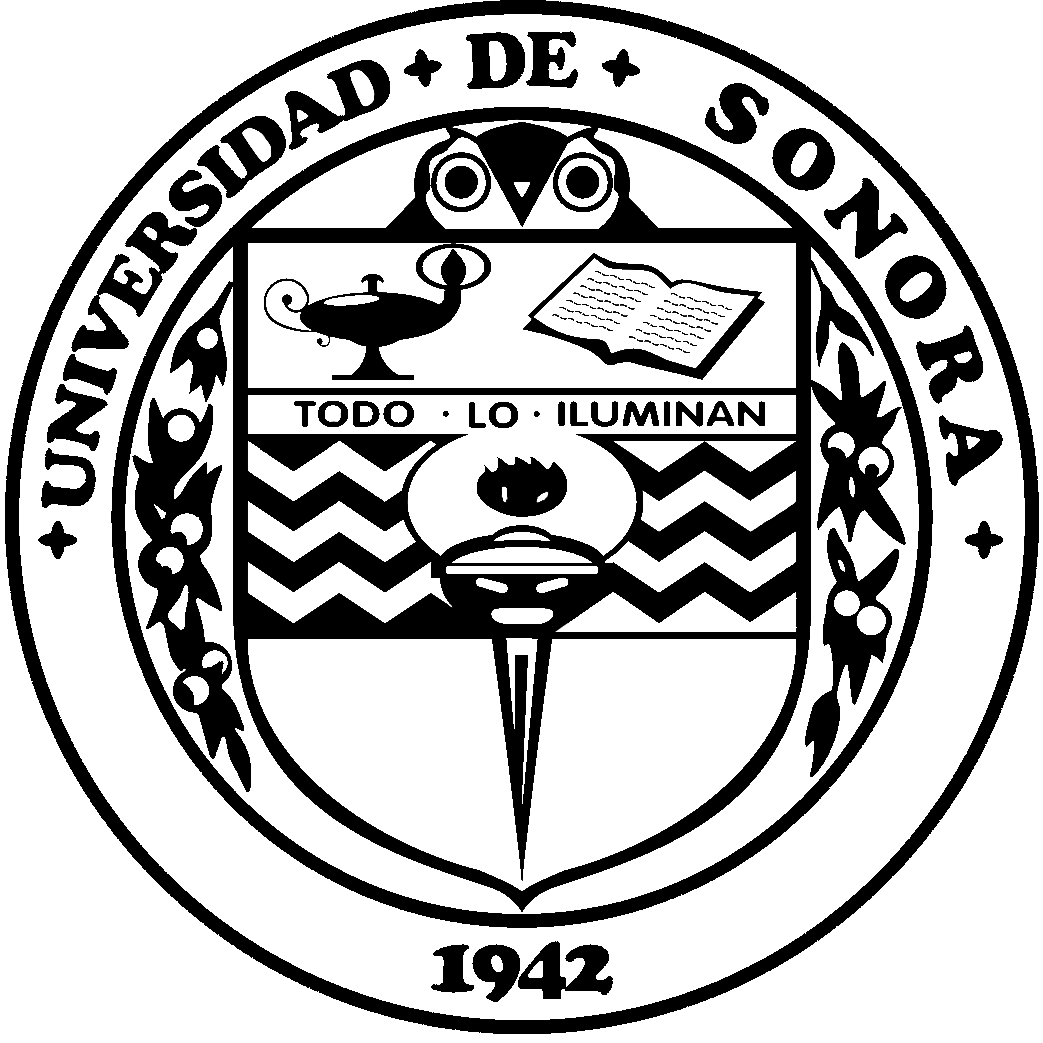
\includegraphics[width=4cm]{escudo.png}

    \vspace{0.5cm}

    {\Large \textbf{Universidad de Sonora}}\\[0.3cm]
    {\large Licenciatura en Ciencias de la Computación}

    \vspace{2cm}

    {\Large \textbf{Generaciones de las Computadoras}}\\[0.3cm]
    {\large Investigación documental y reporte}

    \vspace{2cm}

    \begin{tabular}{rl}
        \textbf{Materia:} & Redes de Computadoras I \\[4pt]
        \textbf{Periodo:} & 2026-2 \\[4pt]
        \textbf{Profesor:} & Dr. Donald José Rodríguez Úbeda \\
    \end{tabular}

    \vspace{1.5cm}

    {\large \textbf{Integrantes del equipo}}

    \vspace{0.4cm}

    \begin{tabular}{ll}
        Angel Fernando Bórquez Guerrero & Expediente 219208106 \\[4pt]
        Angel Alberto Amaya Soria & Expediente 223210350 \\[4pt]
        Javier Leonardo Miranda Sánchez & Expediente 223215039 \\[4pt]
        Oliver Ruiz Beltrán & Expediente 223204115 \\
    \end{tabular}

    \vfill

    {\large Hermosillo, Sonora \hspace{1cm} Agosto de 2026}

\end{titlepage}

% ==================================================
% ÍNDICE
% ==================================================
\tableofcontents
\newpage

% ==================================================
% CONTENIDO
% ==================================================
\section{Introducción}

El presente reporte tiene como objetivo investigar y describir las distintas generaciones en las que tradicionalmente se clasifica la evolución histórica de las computadoras. Para cada generación se analizan los componentes electrónicos empleados en su construcción, las características de hardware que la distinguen, los dispositivos de entrada y salida disponibles, los lenguajes de programación utilizados, el software de base existente (sistemas operativos, compiladores e intérpretes) y el uso que se les daba a los equipos de la época. Conocer esta evolución permite comprender cómo los avances en la electrónica han impulsado, en cada etapa, mejoras en la velocidad, el tamaño, el costo y las aplicaciones de las computadoras.

\section{Generaciones de las computadoras}

\subsection{Primera generación (1940--1956)}

\textbf{Componentes utilizados para su construcción.} Las computadoras de esta generación se construyeron con tubos de vacío (bulbos) como elemento básico de conmutación, y empleaban tambores magnéticos o líneas de retardo de mercurio como memoria principal.

\textbf{Características de hardware.} Eran equipos de dimensiones enormes, capaces de ocupar habitaciones o sótanos completos, con pesos de varias toneladas; consumían grandes cantidades de energía eléctrica y generaban mucho calor. Los tubos de vacío se fundían con frecuencia, lo que provocaba fallas constantes y baja fiabilidad. Su velocidad de cálculo era muy limitada en comparación con las generaciones posteriores, y solo podían ejecutar una operación a la vez.

\textbf{Dispositivos de entrada/salida.} La entrada de datos y de instrucciones se realizaba principalmente mediante tarjetas perforadas y cintas de papel perforado; en algunos casos también se empleaba cableado físico en tableros de conexión. La salida se obtenía por medio de tarjetas perforadas o de impresoras rudimentarias.

\textbf{Lenguajes de programación.} Se programaban directamente en lenguaje máquina, es decir, mediante instrucciones binarias específicas de cada equipo, e incluso mediante la reconexión física de cables y tableros para configurar cada nuevo programa.

\textbf{Software de base disponible.} No existía todavía un sistema operativo como tal. Cada programa se cargaba y ejecutaba de forma manual por un operador humano, que introducía las tarjetas o cintas correspondientes y esperaba a que el trabajo terminara antes de iniciar el siguiente. Al no existir lenguajes de alto nivel, tampoco existían compiladores ni intérpretes.

\textbf{Utilización.} Estas máquinas se emplearon casi exclusivamente con fines militares, científicos y gubernamentales, por ejemplo en el cálculo de tablas de tiro de artillería y en labores de criptoanálisis, siendo operadas por personal altamente especializado en instituciones y universidades.

\subsection{Segunda generación (1956--1964)}

\textbf{Componentes utilizados para su construcción.} El elemento distintivo de esta generación fue el transistor, que sustituyó al tubo de vacío como componente de conmutación; la memoria principal comenzó a construirse con núcleos de ferrita magnética.

\textbf{Características de hardware.} Gracias al transistor, las computadoras redujeron considerablemente su tamaño, su consumo eléctrico y el calor generado, además de volverse más rápidas y confiables que las de la primera generación. Aun así, seguían siendo equipos costosos, instalados en salas especialmente acondicionadas y operados por personal profesional.

\textbf{Dispositivos de entrada/salida.} Continuaron utilizándose las tarjetas perforadas como medio principal de entrada, y comenzaron a emplearse cintas magnéticas para el almacenamiento y transporte de datos entre equipos; la salida se obtenía mediante impresoras de línea.

\textbf{Lenguajes de programación.} Además del lenguaje ensamblador, surgieron los primeros lenguajes de programación de alto nivel: FORTRAN, orientado a cálculos científicos, y COBOL, orientado a aplicaciones administrativas y de negocios.

\textbf{Software de base disponible.} Aparecieron los primeros sistemas operativos sencillos de procesamiento por lotes (\textit{batch}), consistentes en un pequeño monitor residente en memoria que automatizaba la carga y ejecución secuencial de los trabajos, evitando que un operador tuviera que intervenir entre cada uno. Surgieron también los primeros compiladores para FORTRAN y COBOL, que facilitaron enormemente la tarea de programar, aunque complicaron la operación de la máquina, ya que cada trabajo requería pasos diferenciados como cargar la cinta del compilador, ejecutar la compilación y después ejecutar el programa resultante.

\textbf{Utilización.} Se mantuvo el uso científico y militar, pero comenzó a extenderse de forma importante el uso empresarial y administrativo, por ejemplo en cálculo de nóminas, contabilidad y procesamiento de datos comerciales.

\subsection{Tercera generación (1964--1971)}

\textbf{Componentes utilizados para su construcción.} El avance característico de esta generación fue el circuito integrado, una pastilla de silicio (chip) capaz de reunir numerosos transistores y otros componentes electrónicos en un solo elemento.

\textbf{Características de hardware.} Los equipos redujeron aún más su tamaño y consumo, al tiempo que aumentaron notablemente su velocidad y fiabilidad. Surgieron familias de computadoras compatibles entre sí, como la IBM System/360, que permitían ejecutar el mismo software en distintos modelos, así como las primeras minicomputadoras, más pequeñas y económicas que los grandes mainframes.

\textbf{Dispositivos de entrada/salida.} Se incorporaron terminales interactivos con teclado y pantalla, que permitían a los usuarios comunicarse directamente con la computadora; también se emplearon discos magnéticos como medio de almacenamiento, además de las tarjetas perforadas y las impresoras, que seguían en uso.

\textbf{Lenguajes de programación.} Se consolidó el uso de FORTRAN y COBOL, y aparecieron nuevos lenguajes de alto nivel como BASIC, pensado para facilitar el aprendizaje de la programación, y PL/I.

\textbf{Software de base disponible.} Se desarrollaron sistemas operativos de multiprogramación, capaces de mantener varios programas en memoria principal al mismo tiempo y repartir el uso del procesador entre ellos, así como los primeros sistemas de tiempo compartido (\textit{timesharing}), que permitían a múltiples usuarios trabajar de forma interactiva y simultánea a través de terminales, dando a cada uno la sensación de tener la máquina completa para sí mismo. Entre los sistemas operativos representativos de esta etapa se encuentran OS/360 y las primeras versiones de UNIX. Los compiladores se volvieron más sofisticados y comenzaron a soportar múltiples lenguajes de alto nivel de forma más eficiente.

\textbf{Utilización.} El uso empresarial se generalizó en sectores como la banca y las líneas aéreas, y las instituciones educativas comenzaron a incorporar computadoras para investigación y docencia; también se popularizó el teleproceso, es decir, el acceso remoto a una computadora central desde terminales distribuidos.

\subsection{Cuarta generación (1971--1981)}

\textbf{Componentes utilizados para su construcción.} El elemento definitorio de esta generación fue el microprocesador, un circuito integrado de alta densidad (tecnología LSI y posteriormente VLSI) capaz de reunir en un solo chip todas las funciones de la unidad central de procesamiento. Las memorias de núcleos magnéticos fueron sustituidas por memorias de semiconductores de tipo RAM y ROM.

\textbf{Características de hardware.} Las computadoras se volvieron mucho más pequeñas, económicas y accesibles, dando lugar a la computadora personal (PC). El primer microprocesador comercial, el Intel 4004, se lanzó en 1971; a partir de entonces la capacidad de procesamiento y la cantidad de memoria disponible crecieron de manera constante mientras el tamaño y el costo de los equipos disminuían.

\textbf{Dispositivos de entrada/salida.} Se generalizó el uso del teclado y el monitor tipo CRT como dispositivos principales de entrada y salida, se incorporaron las unidades de disquete para almacenamiento, y hacia el final de esta generación comenzó a emplearse el ratón (\textit{mouse}); las impresoras matriciales se volvieron comunes en el entorno doméstico y de oficina.

\textbf{Lenguajes de programación.} Se popularizaron lenguajes de alto nivel como C y Pascal, además de versiones interpretadas de BASIC integradas directamente en muchas microcomputadoras; también comenzaron a surgir los primeros lenguajes orientados a objetos, como Smalltalk.

\textbf{Software de base disponible.} Surgieron los primeros sistemas operativos pensados para computadoras personales, como 86-DOS y posteriormente MS-DOS, basados en una interfaz de línea de comandos monousuario; en paralelo, para minicomputadoras y redes de equipos se desarrollaron sistemas operativos distribuidos y en red. Se popularizaron los intérpretes de BASIC, así como compiladores de C y Pascal, y comenzó a surgir software de aplicación de base como procesadores de texto y hojas de cálculo.

\textbf{Utilización.} Nació el uso personal y doméstico de la computadora, que se extendió también a oficinas pequeñas, escuelas y hogares, democratizando el acceso a la informática, que hasta entonces había estado reservado a grandes instituciones.

\subsection{Quinta generación (1981/1982--actualidad)}

\textbf{Componentes utilizados para su construcción.} Esta generación se caracteriza por el uso de circuitos de integración a muy gran escala (VLSI) y a ultra gran escala (ULSI), así como por microprocesadores con múltiples núcleos y memorias de estado sólido.

\textbf{Características de hardware.} Los equipos son cada vez más pequeños, portátiles, potentes y económicos; se incorpora el procesamiento en paralelo, avances en tecnología de superconductores y una conectividad de red prácticamente universal gracias a Internet. Además de las computadoras de escritorio y portátiles, esta generación incluye tabletas y teléfonos inteligentes con gran capacidad de cómputo.

\textbf{Dispositivos de entrada/salida.} Además del teclado y el ratón, se generalizan las pantallas táctiles, el reconocimiento de voz y de rostro, las cámaras integradas y diversos sensores, así como impresoras láser y de inyección de tinta de alta resolución.

\textbf{Lenguajes de programación.} Se emplean lenguajes de alto nivel modernos orientados a objetos y de propósito general, como Java, Python, C++ y JavaScript, así como lenguajes y herramientas especializadas en inteligencia artificial y procesamiento del lenguaje natural.

\textbf{Software de base disponible.} Predominan los sistemas operativos gráficos, multiusuario y multitarea, tanto para computadoras de escritorio (Windows, macOS, distribuciones de Linux) como para dispositivos móviles (Android, iOS), además de sistemas operativos distribuidos y en red que permiten compartir recursos entre múltiples equipos interconectados. Los compiladores e intérpretes modernos incorporan técnicas de compilación en tiempo de ejecución (\textit{just-in-time}) y se apoyan en entornos de desarrollo integrados (IDE) que facilitan la programación en múltiples lenguajes.

\textbf{Utilización.} El uso de las computadoras se ha vuelto masivo en los ámbitos personal, empresarial y educativo, impulsado por Internet, las redes sociales, la computación en la nube y el desarrollo de la inteligencia artificial, que permite que los equipos incorporen funciones de aprendizaje automático y reconocimiento de patrones en tareas cotidianas.

\section{Conclusión}

El estudio de las generaciones de las computadoras muestra una evolución constante impulsada principalmente por los avances en la electrónica: del tubo de vacío al transistor, de este al circuito integrado y finalmente al microprocesador con integración a muy gran escala. Cada avance en los componentes trajo consigo equipos más pequeños, rápidos, confiables y económicos, lo que a su vez permitió el desarrollo de sistemas operativos y lenguajes de programación cada vez más sofisticados, así como una ampliación progresiva de los usos de la computadora: de las aplicaciones científicas y militares exclusivas de la primera generación, se pasó al uso empresarial, personal y finalmente masivo que caracteriza a la quinta generación actual.

% ==================================================
% REFERENCIAS BIBLIOGRÁFICAS (formato APA)
% ==================================================
\newpage
\section*{Referencias bibliográficas}
\addcontentsline{toc}{section}{Referencias bibliográficas}

\begin{itemize}[leftmargin=1.5em,itemsep=8pt]

\item[] Belmonte Vesga, A. J. (2024, octubre 8). \textit{Historia de los sistemas operativos en 20 minutos o más}. Medium. \url{https://medium.com/@belmontevesga/historia-de-los-sistemas-operativos-en-20-minutos-o-mas-edc670fc5d9a}

\item[] Diferenciador. (2021, junio 23). \textit{Generaciones de computadoras: cuántas hay, características y ejemplos}. \url{https://www.diferenciador.com/generaciones-de-computadoras/}

\item[] Enciclopedia Concepto. (2025, agosto 19). \textit{Generaciones de las computadoras}. \url{https://concepto.de/generaciones-de-las-computadoras/}

\item[] Enciclopedia Significados. (2025, julio 17). \textit{Generaciones de computadoras: cuántas hay, características e historia}. \url{https://www.significados.com/generaciones-de-computadoras/}

\item[] Euroinnova. (2026, julio). \textit{¿Qué son las generaciones de la computadora?} \url{https://www.euroinnova.com/blog/que-son-las-generaciones-de-la-computadora}

\item[] Mateu, L. (s.f.). \textit{Historia de los Sistemas Operativos}. Universidad de Chile. \url{https://users.dcc.uchile.cl/~lmateu/CC41B/Apuntes/evolucion/historia.htm}

\item[] Universidad del Valle de México, Campus Sur. (s.f.). \textit{Historia de los Sistemas Operativos}. \url{https://sites.google.com/site/sistemasoperativosuvmsur/historia-de-los-sistemas-operativos}

\item[] Wikipedia. (2026, julio 7). \textit{Generaciones de computadoras}. En \textit{Wikipedia, la enciclopedia libre}. \url{https://es.wikipedia.org/wiki/Generaciones_de_computadoras}

\end{itemize}

\end{document}
